\documentclass[12pt]{article}
\usepackage[utf8]{inputenc}
\usepackage[russian]{babel}
\usepackage[margin=1.5in,left=1cm,right=1cm, top=2cm,bottom=2cm,bindingoffset=0cm]{geometry}
\usepackage{graphicx}
\usepackage{color}
\usepackage{amssymb}
\usepackage{minted}
\usepackage{hyperref}
\usepackage{amsmath}
\usepackage{fancyhdr}



\title{Title}
\author{Амеличев Константин, ПМИ 191.}
\date{Date}

\newcommand{\problem}[2]{

\section {Задача #1}
\textbf {Постановка задачи.} {#2}

\textbf {Решение.}
}

\newcommand{\limit}[2]{\displaystyle \lim_{#1 \to #2}}

\newcommand{\rangesum}[2]{\displaystyle \sum_{#1}^{#2}}

\newcommand{\mintedparams}{
% frame=lines
% framesep=2mm,
% baselinestretch=1.2,
% bgcolor=LightGray    
}

\pagestyle{fancy}
\fancyhf{}
\fancyhead[LE,RO]{Амеличев Константин, ПМИ 191, @kik0s, \href{http://github.com/kik0s}{\textcolor{blue}{github}}, \href{http://codeforces.com/profile/kikos}{\textcolor{blue}{codeforces}}, \href{http://vk.com/i_tried_to_name_myself_kikos}{\textcolor{blue}{vk}}}
\fancyhead[RE,LO]{Лекция АиСД 27.11}

\begin{document}

\paragraph{Больше куч!}

\begin{center}
\begin{tabular}{c|c|c|c}
&$binary heap$ & $binomial heap$ & $fibonacci heap$ \\
$insert$ & $O(\log n)$ & $O(\log n)$ & $O(1)$\\
$extract\_min$ & $O(\log n)$ & $O(\log n)$ & $\tilde O(\log n)$\\
$decrease\_key$ & $O(\log n)$ & $O(\log n)$ & $\tilde O(1)$\\
$increase\_key$ & $O(\log n)$ & $O(\log n)$ & $\tilde O(\log n)$\\
$merge$ & $\tilde O(\log^2 n)$ & $O(\log n)$& $O(1)$\\
$get\_min$ & $O(\log n)\ or\ O(1)$ & $O(1)$ 
\end{tabular}
\end{center}

\paragraph{Биномиальная куча}
\hspace{\fill}

Храним биномиальные деревья. Каждому дереву сопоставим ранг. Ранг дерева полностью определяет его структуру. Дерево ранга 0 --- одна вершина. Дерево ранга 1 --- одно ребро. В общем случае, дерево ранга $n$ содержит корень и полное двоичное дерево размера $2^{n-1}$. Дерево ранга $n+1$ --- это два слитых вместе дерева ранга $n$ --- корень второго указывает на корень первого, а корень первого теперь будет указывать на оба бинарных дерева.

Биномиальная куча --- это набор из логарифма биномиальных куч.

Слияние двух деревьев мы научились делать за $O(1)$ --- меньшая вершина по ключу становится новым корнем, а дальше перекидываем указатели.

Слияние двух куч --- это алгоритм сложения двоичных чисел --- при сливании двух деревьев ранга $n$ мы <<переносим>> прибавление кучи ранга $n+1$

Как добавлять элемент? Создать кучу на 0 элементов и слить их вместе.

Уменьшение ключа --- напишем $sift\_up$ на нашей новой куче

Удаление минимума --- Заметим, что если в правом дереве пройти по правым детям и обозначим их за корни, а их левых детей за полные бинарные деревья, то мы получим набор деревьев рангов $0, 1, \dots, n - 1$. Обозначим их за новую кучу, и сольем все вместе.

Увеличение ключа --- удалим соответствующий элемент и добавим другой.

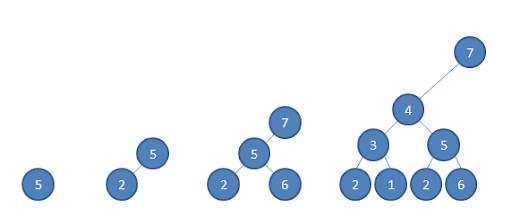
\includegraphics{pictures/binoial_heap.png}
\newpage
\paragraph{Фибоначчиева куча}
\hspace{\fill}

Хотим сделать биномиальную кучу с послаблаблениями --- делать операции в самый последний момент, менее четкую структуру, etc

Есть деревья, их корни храним в двусвязном закольцованном списке.

Всех детей для всех вершин храним в двусвязном закольцованном списке.

Новый ранг --- это количество вершин в списке детей.

На каждом дереве выполнена куча, а также поддерживаем глобальный минимум.

Улучшение ключа делается так --- удаляем вершину из своего списка, вместе с поддеревом. Добавляем в корневой список. Если мы удалили уже вторую вершину в поддереве родителя, то делаем каскадное вырезание --- прыгаем по предкам с $mark = 1$, и вырезаем их в корневой список, причем все вырезания делаются по очереди.

Удаление делается так --- мы приписываем всех детей к корневому списку, а потом вызываем $compact$, которая должна спасти наше дерево и навести порядок.

Псевдокод тупых операций:
\begin{minted}{c++}
    struct Node{ 
        Node *child;
        Node *left;
        Node *right;
        Node *parent;
        int rank;
        bool mark;
        int value;
    }

    list<Node *> roots;

    void insert(int x) {
        Node *node = new Node(x);
        roots.insert(node);
    }

    void merge(list<Node *> a, list<Node *> b) {
        merge(a, b); // O(1) haha super easy
    }

    int getmin() {
        return argmin->value;
    }
\end{minted}

\paragraph{compact} 
\begin{itemize}
\item Сбрасываем пометки корневого списка в 0
\item Переводим дерево в состояние, где все ранги разлиичны
\item Храним ранги, мерджим одинаковые
\item Как мерджим? Берем меньший корень, и записываем в его детей второй корень
\end{itemize}

Обозначим $R = \max rank$, $t(H) = root\ list\ size$, $m(H) = \sum_{v} mark(v)$

$compact$ работает за $O(R + t(H))$.

\paragraph{Анализ времени работы}

$extract\_min\ \& increase\_key$ --- $\tilde O(R)$.

$\Phi(H) = t(H) + 2m(H) < 3n$

Пусть каскадное вырезание сделало $t_i $ действий. $m:\ 1 \rightarrow 0,\ t:\ +1$. Тогда $\Phi'(H) = \Phi(H) - 1$ за каждое вырезание.
Тогда амортизированно вырезание работает за $O(1)$.

Compact:

$t(H) \le R$, $t'(H) = t(H) - R$

Амортизациованно работает за $2R + 1$

Хотим показать $R = O(\log n)$.

$$\forall\ v \in H\ sz(v) \ge A^{rank(v)},\ A > 1$$

Тогда 

$$r(v) \le \log_A s(v) \le c \log n$$

Возьмем

$$s(v) \ge \phi^{rank(v) - 2}$$

\textit{<Оффтоп про числа Фибоначчи>} 
\begin{enumerate}
    \item $F_n = F_{n - 1} + F_{n - 2},\ F_0 = F_1 = 1$ 
    \item $F_n \ge \phi^{n - 2}$
    \item $\forall\ i \ge 2:\ F_i = \rangesum{j=0}{i-2}F_j + 1$
\end{enumerate}
\textit{</Оффтоп про числа Фибоначчи>} 

Почему инвариант на размеры сохраняется? Возьмем вершину $v$ с $k$ детьми. Рассмотрим детей в том порядке, в котором их склеивал компакт. Тогда на момент добавления $i$-й вершины в структуру, ее ранг совпадал с рангом $v$. Тогда из условия на удаление не более чем одного сына ($mark$) следует, что $rank(i) \ge i - 1$. Тогда мы доказываем по индукции, что у нас все размеры --- хотя бы числа фибоначчи, соответствующие рангу. Тогда $s(v) = \sum_{u \in g(v)} s(u) + 1 \ge \sum_{u \in g(v)} F_rank(u) + 1 \ge \rangesum{i=0}{rank(v) - 2}F_{i} + 1 \ge F_{rank(v) - 2}$



\end{document}
